\section{Introduction}
Outsourcing the storage of and computation over private data to cloud service
providers~\cite{amazon_aws,microsoft_sql,monogb_sql,google_sql} 
is a common practice for personal users, enterprises, and even government
institutions to lift the burden of large-scale data management.
However, in many cases, the outsourced data contain sensitive information, and
data owners are concerned with their private data either
directly stolen by the curious cloud service providers~\cite{lu2019assessing} or 
leaked through the endless data breaches~\cite{trautman2017corporate,
cadwalladr2018revealed}.  As a result, data owners
and cloud service providers are interested in building encrypted 
database infrastructures~\cite{poddar12arx}, where the entire database is stored 
in ciphertext on the cloud. 
However, due to the inherent complexity in the design
of multi-party secure protocols, 
the fundamental challenge confronting encrypted databases is on how to efficiently 
and elastically process queries on the encrypted data outsourced to the cloud while preventing 
various side channel leakages~\cite{cash2015leakage,grubbs2018pump, attackSOD}.
% What the past decade witnessed is a period of fast development in database
% management systems (DBMS) as a cloud-based service, which provides not only
% data storage and queries, but also business operational analytics and machine
%learning (ML) predictions to get a deeper insight into data
% However, such cloud-based DBMS requires users to provide their sensitive data, 
% like financial transactions and medical records, and may lead to data breaches due
% to the cyber-attacks or the illegal use of data by database administrators (DBA).
% Give rise to encrypted database


% Unfortunately, many of the above protocols are designed to be {\it{application-specific}}.
% In other words, due to security, data compatibility, and efficiency reasons, 
% it can be challenging to combine different database functionalities
% into a unified framework.

\begin{figure}[t!]
   \begin{center}
   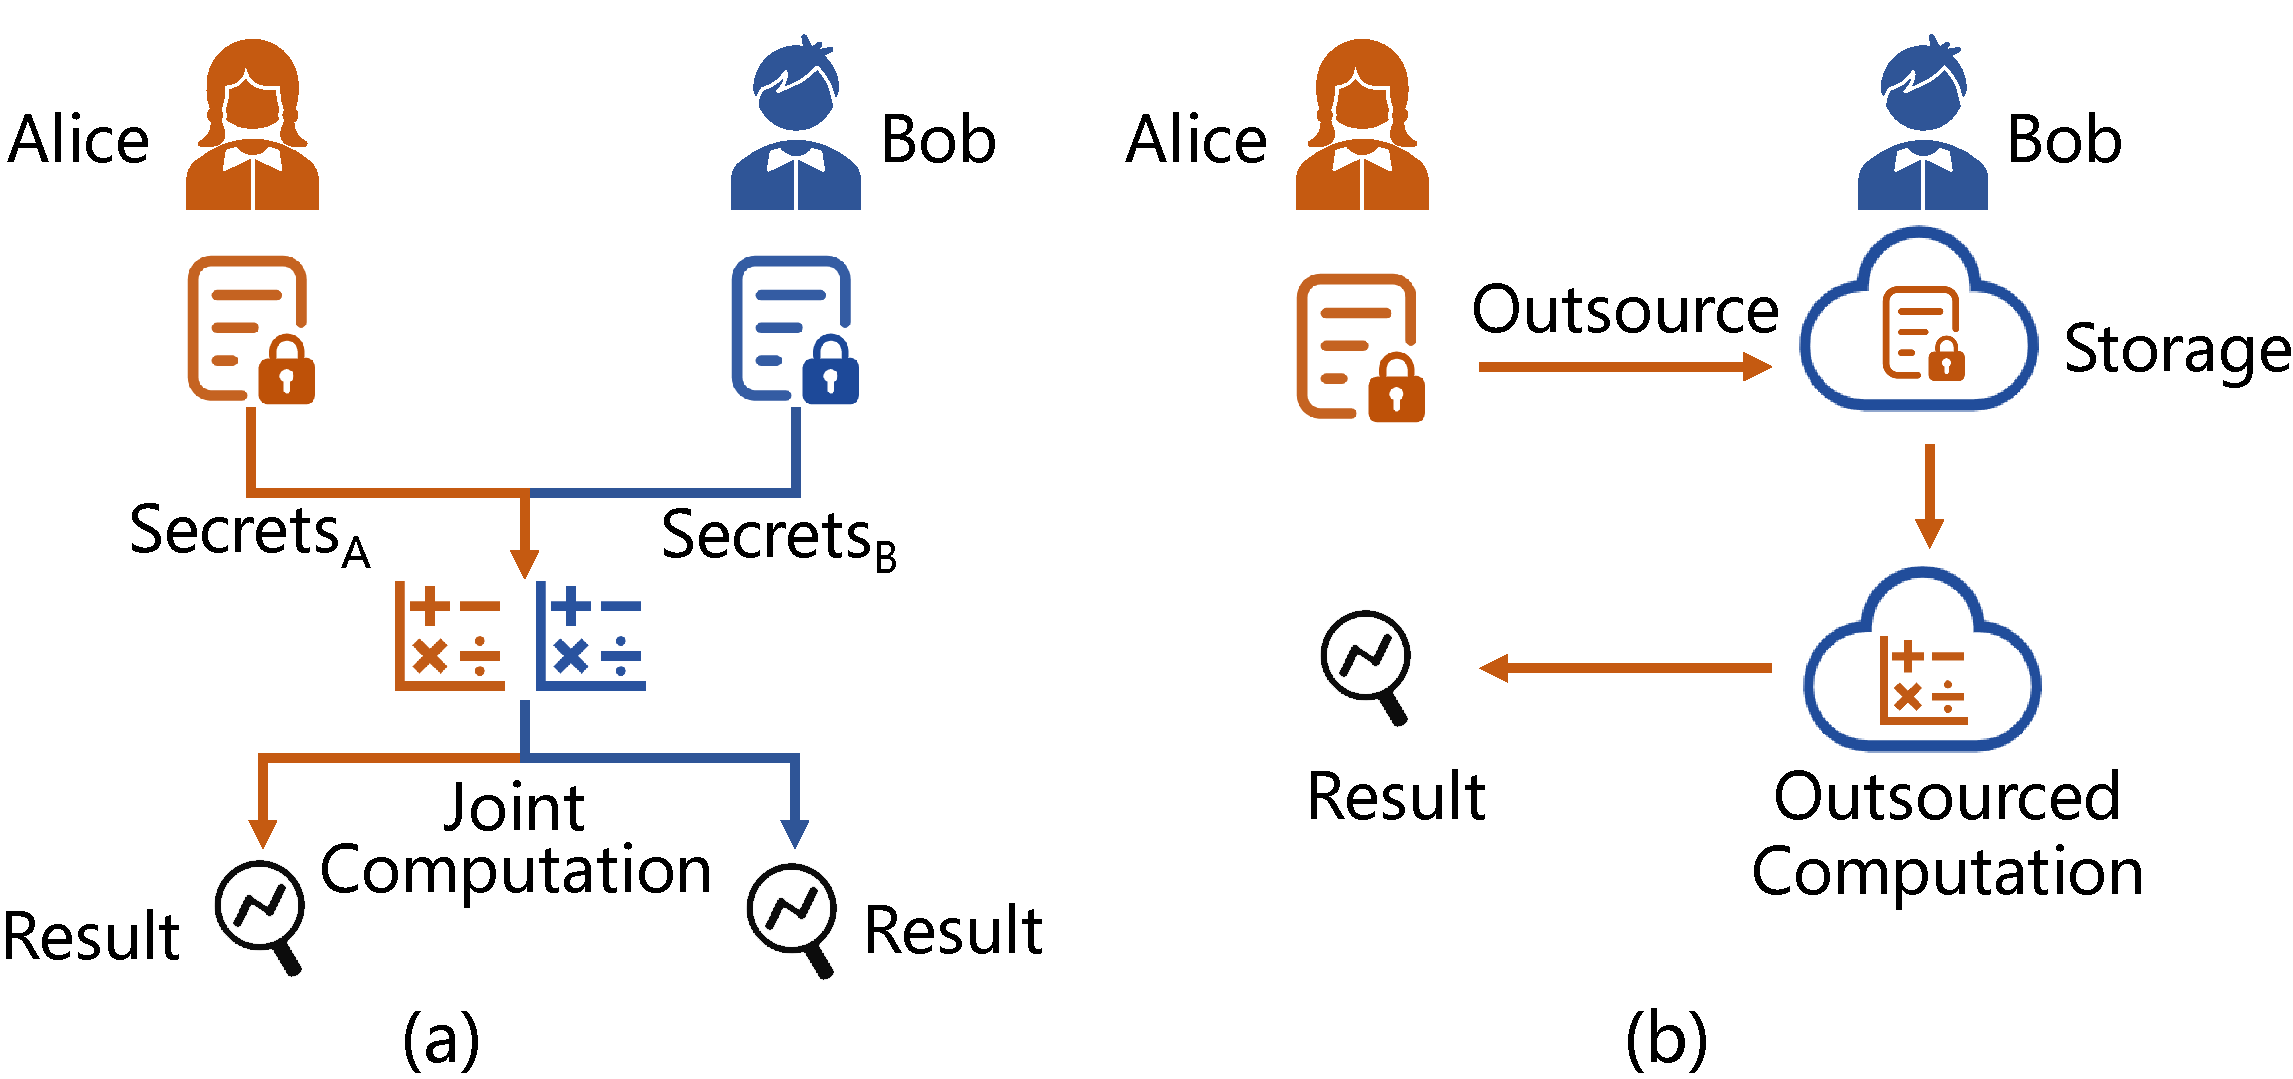
\includegraphics[width=1\linewidth]{figure/sdonsqe.pdf}
   \end{center}
      \caption{The conceptual illustrations of (a) a secure
      multi-party query evaluation (SQE) scheme and (b) a
      secure database outsourcing (SDO) scheme.} 
   \label{fig:threat}
   % \vspace{-0.5em}
\end{figure}

To tackle the above challenges, existing works propose different designs of encrypted
databases that utilize tools across multiple fields of 
research~\cite{sagma,eskandarian2017oblidb,priebe2018enclavedb,esolute,yi2012single,wang2021secure,liagouris2021secrecy,poddar2021senate,waldo,heda}.
% Depending on the targeting threat model, encrypted databases
% are constructed over a plethora of cryptographic or secure computing methods, 
% including those based on
% oblivious random access machine (ORAM)~\cite{oblidb}, searchable encryption 
% (SE)~\cite{sagma}, trusted execution environment 
% (TEE)~\cite{eskandarian2017oblidb,priebe2018enclavedb}, differential privacy~\cite{esolute}, 
% private information retrieval~\cite{yi2012single}, private set intersection~\cite{wang2021secure}, 
% and secure multi-party computing  (MPC)~\cite{liagouris2021secrecy, poddar2021senate, waldo, heda}.
We categorize existing designs of encrypted databases
into two types of protocol models: secure multi-party query evaluation (SQE) and 
secure database outsourcing (SDO).
% encrypted databases 
% by whether hardware trusted execution environment (TEE) is adopted and 
% whether the presumed threat model is .  
As illustrated in \cref{fig:threat}, we assume that no party 
in an SQE protocol can recover all of the secrets only by its own.
In contrast, SDO refers to the case where one of the participating parties 
(e.g., the one who outsources the data) owns all of the private data. 
Thus, even though both SQE and SDO prefer lower
protocol overheads, parties involved in SQE are willing to pay more
computation and communication costs in the exchange of being
able to compute over unknown secrets. Meanwhile, for SDO, client-side workloads need
to be strictly smaller than that without the protocol, otherwise the client
can simply perform the computations locally on its own.
% SDO is defeated.

With the optimal round complexity~\cite{mukherjee2016two} and
low online communication, fully homomorphic encryption (FHE) 
emerges as a powerful cryptographic primitive for SDO.
% Since arbitrary computations can be executed on the homomorphically encrypted 
While FHE was deemed too slow to DB applications~\cite{shan2018practical}, 
recent advances in FHE 
cryptography~\cite{conversionhaochen, revisiting, pegasus, meta-bts}
have significantly improved the efficiency and operator usability of FHE,
leading to a series of recent works exploring the practical feasibility
of FHE in DB-related tasks~\cite{pegasus,cong2021labeled,heda}.
For instance, the very recent work HEDA~\cite{heda} employs FHE schemes including the 
BFV~\cite{DBLP:conf/crypto/brakerski12,DBLP:journals/iacr/FanV12} and 
TFHE~\cite{DBLP:journals/joc/ChillottiGGI20}  
to accelerate filter-aggregation queries over fully homomorphically 
encrypted database. Unfortunately, in addition to the relatively
slow evaluation speed, HEDA suffers from limited query expressiveness
% the computational costs of HEDA remain relatively high as a single ciphertext 
% format conversion 
% from the filtering mode to the aggregation mode requires 9 seconds~\cite{heda},
% which translates to a query latency of more than 100 days over a DB with one 
% million rows. In addition, as mentioned in~\cite{heda},
as the exact algorithmic constructions for the evaluations of many 
common SQL statements, such as $\dbmin$, $\dbmax$, $\join$ and $\orderby$,
are left as open questions~\cite{heda}. %, limiting the query expressiveness of HEDA.
% Data analysis capabilities 
% to be performed on the aggregated results, due to the lack of efficient homomorphic
% conversion algorithms. 
Therefore, the main challenge faced by FHE-based SDO becomes the following question:
can we design an encrypted database scheme over FHE that achieves both fast query 
evaluation and elastic data processing at the same time?
% Therefore,
% despite that homomorphic encryption (HE) has been traditionally employed in building
% both SQE~\cite{chen2017fast,poddar2021senate} and 
% SDO~\cite{cryptdb, poddar12arx,sagma,aphadb},
% most designs only adopts partially or leveled homomorphic encryption schemes instead
% of adopting an FHE setup. However, along with the 
% FHE-based encrypted database 
\subsection{Our Contribution}
In this work, we propose \NAME, 
an FHE-based encrypted DBMS for fast and elastic SDO. 
We observe that most existing FHE algorithms, 
whether specifically designed for SDO~\cite{heda} or not~\cite{pegasus,ckkscomparison}, 
do not fully capture the important properties of encrypted databases,
and often fail to meet the key requirements of SDO.
%Different from the general FHE algorithms suggested by existing work,
Contrarily, based on the idea of application-framework co-design, 
we propose a tailored FHE infrastructure consisting of DB-specific
FHE operators that leverage the numerical and operational characteristics
specific to encrypted databases. As it turns out, we are able to
achieve higher accuracy, faster evaluation speed, richer query expressiveness
and better security all at once.
% By devising a set of new cryptographic 
% tools, \NAME is able to evaluate one of the most complete sets
% of SQL statements under an SDO setting, at speeds that are $10$--$100\times$ faster
% than the respective existing solutions. 
In addition, to the best of our knowledge,
\NAME is the first FHE-based DB framework that enables a client to
execute outsourced data analysis algorithms on the queried ciphertext results 
without additional rounds of client-server 
interactions.
% , which is a key feature for many outsourced DBMS that is
% missing in existing solutions~\cite{heda}.
%, using complex learning algorithms such as private decision tree. 

% The main contributions of this work are summarized as follows.
% that achieves low computation cost and storage in the DBMS 
% provider and unbound number of filtering predicates and aggregations analysis. 
% outsourced, complete, 

% \vspace{0.03in}
\noindent
\begin{itemize}
    \item {\bf{An FHE Infrastructure for Encrypted DBMS}}:
    % We decompose the SQL queries into a set of fundamental arithmetic and 
    % logic functions, and design DB-specific FHE operators to efficiently 
    % realize such functions.
    We develop novel homomorphic filtering, aggregation and
    conversion algorithms that are highly composable and specifically designed
    for various types of DB operands and complex SQL operations.
    As a result, \NAME supports one of the most complete sets 
    of SQL statements 
    for encrypted databases, along with online data analysis capability.
    % , including unbounded-depth filter-aggregation, grouping, sorting,
    % and joining of encrypted DB items. 
    % a new FHE infrastructure needs to be constructed to handle the complex 
    % queries over databases. 
    % In particular, multiple FHE ciphertext formats need to 
    % co-exist,  and efficient conversion algorithms need to be installed .
    %FHE -> algorithm -> framework
    \item {\bf{High-Precision Homomorphic Comparison}}: 
    We observe that, the key FHE operator for encrypted database is
    the high-precision homomorphic comparison operator. 
    However, the result of a homomorphic comparison is always binary.
    Based on the above insight, we devise a new shift-and-subtract strategy
    to homomorphically remove the lower-bit noises from the comparison results,
    and develop a high-precision homomorphic comparison operator $\homcomp$.
    %by subsequent DB aggregations. 
    %Our $\homcomp$ operator can
    We can evaluate homomorphic comparison with up to 32-bit precision without using
    bit-by-bit encryption.
    % and are able to carry out
    % fast homomorphic comparisons between inputs that are both ciphertexts encrypting
    % up to 32-bit precision plaintext messages, without relying on bit-by-bit encryption.
    %achieving the highest level of accuracy to the best of our knowledge.
    % We obtain high precision comparison by iterating lower precision comparison.
    \item {\bf{Homomorphic Aggregations over Filtered Results}}:
    Based on the $\homcomp$ operator, we are able to propose fast algorithms to perform both 
    arithmetic (e.g., $\dbsum$, $\dbavg$)  and logic (e.g., $\dbmin$, $\dbmax$)
    aggregations on the filtered results. Our arithmetic and logic aggregation
    can be as much as $58\times$ and $34\times$ faster than existing works, respectively.
    % We note that most existing FHE-based DB designs~\cite{yi2012single,aphadb,heda}
    % do not simultaneously support arithmetic and logic aggregations
    
    %arithmetic and logic aggregation, efficient
    
    \item {\bf{Thorough Experiments}}: 
    We show that \NAME achieves $7\times$--$113\times$ faster homomorphic
    filtering, $23\times$--$58\times$ faster homomorphic aggregation,
    $34\times$ faster $\orderby$, and $12\times$--$326\times$ 
    faster private decision tree evaluation, 
    all against the best-performing implementations. In addition,
    we show that \NAME is on average $41\times$--$299\times$
    faster than the state-of-the-art FHE-based DBMS over end-to-end SQL benchmarks. 
    A demo for the 
    end-to-end TPC-H~\cite{tpc_h} query evaluation process is submitted as a 
    proof-of-concept artifact for the proposed algorithms.
    % We plan to provide
    
    % a fully open source implementation \NAME\footnote{A demo of the 
    % end-to-end TPC-H~\cite{tpc_h} query evaluation process is submitted as a proof-of-concept artifact 
    % for the proposed algorithms.}.
\end{itemize}

\subsection{Related Works}\label{sec:relatedworks}
Here, we introduce existing works based on three main groups: 
trust-execution-environment-(TEE)-based SQE and SDO, 
MPC-based SQE, and MPC-based SDO. Note that, here, we consider FHE
to be one particular type of general MPC technique.

% {\bf{TEE-based SDO and SQE}}: 
\subsubsection{TEE-based SDO and SQE}
%It is obvious that there are many advantages of adopting
%hardware enclaves in instantiating encrypted databases: high processing speed,
%low communication overheads, high usability and rich query expressiveness. 
%In particular, 
TEE-based solutions can easily realize both
SDO and SQE simultaneously~\cite{bajaj2011trusteddb, arasu2015transaction, zheng2017opaque, 
eskandarian2017oblidb, priebe2018enclavedb, mishra2018oblix, bailleu2019speicher, 
kim2019shieldstore, vinayagamurthy2019stealthdb, antonopoulos2020azure, wang2022operon}. 
For example, although earlier techniques are constrained by the memory hierarchy of 
TEE~\cite{bajaj2011trusteddb,arasu2015transaction, priebe2018enclavedb}, newer 
TEE architectures have largely abandoned memory integrity verification, thereby 
removing the limit on memory size~\cite{johnson2021supporting, feng2021scalable}. 
Subsequently, recent TEE-based techniques~\cite{antonopoulos2020azure, wang2022operon} 
have demonstrated that advanced DBMS can be built over TEE with advanced access control mechanisms.
Unfortunately, TEE-based encrypted databases face two fundamental challenges.
First, the hardware architectural design of TEE can change significantly from one to 
the other, causing security vulnerabilities to be introduced. 
For example, as mentioned in~\cite{wang2022operon}, encrypted database based on Intel 
SGX~\cite{costan2016intel} 
can leak access pattern~\cite{eskandarian2017oblidb}, while that based on application-specific
TEE enclaves~\cite{suh2007aegis} do not.
% Meanwhile, even if the users are aware of the fact that
% the underlying hardware is insecure for their purpose, switching to a different hardware
% architecture can be too costly or even impossible in some highly customized applications.
Second, as a common critique for most privacy-preserving computing tasks 
based on TEE, it can be discouraging for applications that require
a high level of data confidentiality to adopt a hardware root of trust.
% Hence, while countermeasures such as~\cite{eskandarian2017oblidb} exist to reinforce 
% certain security properties of TEE-based solutions, encrypted databases based on
% TEEs can be insufficient to meet real-world data protection needs.
% {\bf{MPC-based SQE}}: 
\subsubsection{MPC-based SQE}
Most MPC-based encrypted databases focus on developing
methods to evaluate queries over contents that are owned by different participating
parties, e.g., ~\cite{bater2016smcql, ishai2016private, 
fuller2017sok, corrigan2017prio, volgushev2019conclave, 
demertzis2020seal, incshrink, liagouris2021secrecy, poddar2021senate, wang2021secure, waldo}. 
Due to the inherent complexity of SQE,  MPC protocols vary significantly in terms of 
their  security assumptions, 
security properties, efficiency, and usability. The main consequence of such a design 
complexity is that protocols tend to be incompatible with each other, and it can be 
very hard to integrate such protocols into a single database framework. 
For instance, the recent encrypted DB protocol Waldo~\cite{waldo} does
not support certain SQL 
operators such as $\groupby$ and $\join$~\cite{waldo}. 
Although many MPC-based protocols, such as Secure 
Yannakakis~\cite{wang2021secure}, Secrecy~\cite{liagouris2021secrecy} and 
Senate~\cite{poddar2021senate}, do support secure $\groupby$ and $\join$ operations, 
these protocols cannot be easily combined together because 
% of the distinct threat models and
% secure computing primitives. Concretely,
Secure Yannakakis~\cite{wang2021secure} is a two-party protocol that utilizes standard
secret sharing, while Waldo and Secrecy assume an honest-majority three-party setting built over
functional secret sharing~\cite{boyle2021function} and replicated secret 
sharing~\cite{araki2017optimized}.
% , while Senate guarantees full malicious security 
% under a many-party (i.e., more than three-party) setting that primarily relies on 
% garbled circuits. 
% Therefore, while MPC-based SQE techniques and frameworks 
% are under active research, the primary research focuses can 
% Therefore, the primary research focuses of MPC-based SQC can
% differ significantly, and it can be highly non-trivial to quantitatively
% compare \NAME to these works. 
In addition, since secrets are defined to be
distributed over the participating parties, MPC-based techniques generally
require a relatively large amount of communication bandwidth and interaction 
rounds~\cite{waldo}. For example, with proper GPU acceleration~\cite{watson2022piranha}, 
communication can be $6\times$--$1000\times$ slower than the computation in 
the state-of-the-art MPC protocols,
becoming the main latency bottleneck.

% {\bf{MPC-based SDO}}: 
\subsubsection{{MPC-based SDO}}
Different from SQE, methods for SDO explore
how to securely and efficiently {\it{outsource}} a database to an untrusted 
server~\cite{cryptdb,seabed,poddar12arx,sagma,aphadb,heda}. 
Existing MPC-based 
SDO schemes generally adopt more than one type of MPC primitives, including
ORAM~\cite{eskandarian2017oblidb}, SE~\cite{poddar12arx, seabed, sagma}, and 
homomorphic encryption~\cite{cryptdb, eskandarian2017oblidb, sagma}.
However, as mentioned earlier, protocols based on SE~\cite{curtmola2006searchable,cash2013highly} 
introduces side-channel
leakages~\cite{islam2012access,cash2015leakage,grubbs2018pump,grubbs2019learning,
gui2019encrypted}.
% which are crucial security vulnerabilities in realizing encrypted databases. 
Meanwhile, albeit ORAM~\cite{stefanov2018path} achieves poly-logarithmic complexity
in oblivious storing and retrieving data items, executing multi-dimensional 
operations over ORAM, such as sorting, incurs extensive communications
and interactions between the data owner and the cloud server that can be prohibitive
in data outsourcing applications. Finally, most MPC-based SDO adopts some sort of
homomorphic encryption, e.g., based on partially homomorphic
encryption~\cite{cryptdb,poddar12arx, seabed, sagma} or 
leveled homomorphic encryption~\cite{aphadb}. Unfortunately, 
without additional MPC primitives, both partially and leveled homomorphic
encryption result in limited query expressiveness 
and data analysis capability,
either due to complex query encoding schemes or {\it{a-priori}} bounds over
the encryption parameters.
% As also pointed out in related literature~\cite{shan2018practical}, 
% while SDO can be considered as a type of multi-party secure protocol, computation 
% outsourcing is fundamentally different from multi-party secure computing in terms of
% its threat model and protocol goal. 

% As a result, except for TEE-based solutions, 
% only a handful of works scrutinized methods to evaluate information-rich SQL 
% queries over outsourced database.  
% Finally, we point out that most SDO protocols are constructed over some sort 
% of homomorphic encryption schemes~\cite{cryptdb,seabed,sagma}. 

% {\bf{FHE-based SQE and SDO}}: 
\subsubsection{FHE-based SQE and SDO}
Different from partially and leveled homomorphic
encryption, FHE~\cite{DBLP:conf/crypto/brakerski12, DBLP:conf/innovations/bgv12, 
DBLP:journals/dcc/SmartV14, DBLP:conf/crypto/GentrySW13, DBLP:conf/eurocrypt/DucasM15,  
DBLP:journals/joc/ChillottiGGI20,  DBLP:conf/asiacrypt/CheonKKS17} 
is capable of evaluating complex queries over both outsourced and 
two-party secure databases\footnote{We note 
that SQE over single-key FHE is limited to a two-party setting, while more
complicated multi-party protocols require further advance in the
development of multi-key FHE schemes~\cite{peikert2016multi,mukherjee2016two,aloufi2021computing}.}.
Since FHE was extremely computationally expensive in the earlier 
days~\cite{cryptdb,shan2018practical},  protocols over FHE often only implement a
small subset of database-related operations, e.g., 
supporting PIR~\cite{yi2012single} or keyword search~\cite{khedr2015shield,oscc} only.
Recently, motivated by the notable progresses made in the development of
fast and flexible FHE primitives~\cite{pegasus, ckksbootvariance}, new FHE-based
SDO schemes are proposed, e.g.,~\cite{heda}. Nonetheless, in addition to the slower 
performance, 
the query expressiveness of \cite{heda} can be rather restricted,
as the scheme does not have support for common SQL statements such as
$\groupby$ and $\orderby$.
%and data analysis capability, diminishing the benefit of adopting FHE.
Hence, the key objective of this work is to significantly boost the 
computational performance of FHE-based encrypted database while retaining the
rich query expressiveness and unbounded data analysis capability of modern DBMS.

% for the computational overheads of FHE were extremely high.
% While recent works hints that improvements in FHE can potentially be 

% As a result,
% relatively heavy interactions and communications between participating parties for
% the exchange of secrets can be inevitable in MPC-based SQE protocols.

% The goal of SDO is solely to outsource the storage of and related processing over 
% private data.  



% As further discussed in \cref{sec:relatedworks}, while TEE-based solutions generally achieve
% superior computation and communication performance, hardware trust roots can be 
% , i.e., 
% the exchange of secrets {\it{must}} happen between parties for the completion of 
% the protocol. 

% That is the server executes queries on encrypted data and provides a 
% cloud-based encrypted database management system (EDBMS).
% The EDBMS can be thought of as a secure two-party computation (TPC) problem
% and a lot of exciting schemes, such as CryptDB~\cite{cryptdb}, 
% Seabed~\cite{seabed}, SAGMA~\cite{sagma}, IncShrink~\cite{incshrink}, and 
% Waldo~\cite{waldo}, are proposed to solve it, using various cryptographic
% primitives including searchable encryption, secret sharing, and differential
% privacy. Another technology frame, including TrustDB~\cite{trustdb}, 
% ObliDB~\cite{eskandarian2017oblidb}, and Oblix~\cite{mishra2018oblix} 
% requires a trusted proxy setting to apply approaches like 
% oblivious RAM (ORAM) and trust execution environment (TEE).

% However, both streamlines of schemes still exist limitations. The first generic 
% multi-party computation (MPC) approach requires the user to participate in the 
% data processing and is not suitable for outsourcing data to the service provider. The ORAM and TEE are more suited to the trusted proxy setting, which is strict in a real-world application. 

% Homomorphic encryption (HE) is a type of cryptographic 
% primitive known for its high computation but low communication costs in
% carrying out secure multi-party computation and secure outsourcing. While there
% are a few recent works that attempt to provide solutions specific to this problem
% based on somewhat homomorphic encryption (SHE) or fully homomorphic encryption (FHE),
% none take \textit{a practical and outsourced approach}, which is crucial for
% addressing the tussle between \textit{generality and efficiency}. On the one hand, many
% recent works focus on
% SHE~\cite{bfv, ckks} for EDBMS~\cite{aphadb, oscc}. While these schemes are encryption parameters 
% predefined to evaluate the limited number of filtering predicates, 
% this approach is 
% not suitable for an outsourced deployment as a new complicated query would require re-encrypted by users.


% While FHE-based encrypted databases generally 
% enjoy provable security against access 
% pattern attacks~\cite{islam2012access,cash2015leakage} and 
% communication volume~\cite{grubbs2018pump,gui2019encrypted}  
% (in the case of filter-aggregation and online data processing) attacks,
% Meanwhile, some encrypted databases based on partially homomorphic
% encryption~\cite{cryptdb, seabed, sagma} or leveled homomorphic encryption~\cite{aphadb}
% either use additional MPC primitives, have limited query expressiveness 
% or cannot perform further data analysis on the queried results.




%\subsection{Motivation and Main Techniques}

% \subsection{Releated Works}
% Here, we provide a brief review of the recent developments in encrypted databases and homomorphic encryption.
% 
% \subsubsection{Encrypted Database}
% MPC , ORAM 
% 
% \subsubsection{Homomorphic Encryption}\label{related:HE}


% two primary challenges encountered by these schemes. The first challenge 
% is the \textit{unbounded filter and aggregation operations}. 
% The second challenge lies in \textit{efficient data processing in encrypted form}.

% % IF HEDA publish, add HEDA
% For example, HEDA is a state-of-the-art scheme of EDBMS using TFHE gate to support 
% unbounded filtering. FHE that can handle both polynomial and non-polynomial
% homomorphic circuits efficiently. 
% research the feasibility of data managing 
% on encrypted databases.
%To add: ORAM and TEE

% \(\epsilon\)psolute\cite{esolute}
% (what is an encrypted database)
% (secure two-party computation, and some approaches)
% (limitations on these approaches)
% (homomorphic approaches: unbounded and bounded, large ciphertexts, 
